\documentclass{beamer}

\mode<presentation>
{
  \usetheme{Frankfurt}
  \usecolortheme{orchid}
  \setbeamercovered{invisible}
  \setbeamertemplate{footline}[frame number]
}

\usepackage[english]{babel}
\usepackage[latin1]{inputenc}
\usepackage{times}
\usepackage[T1]{fontenc}
\usepackage{tikz}
\usepackage{array}
\usepackage{cancel}


\usetikzlibrary{shapes,backgrounds}

\def\multiset#1#2{\ensuremath{\left(\kern-.3em\left(\genfrac{}{}{0pt}{}{#1}{#2}\right)\kern-.3em\right)}}

\def\blue{\color{blue}~}
\def\black{\color{black}~}
\def\bl[#1]#2{\begin{block}{#1}#2\end{block}}
\def\integers{\mathbb{Z}}
\def\enumb{\begin{enumerate}}
\def\enume{\end{enumerate}}
\def\itemb{\begin{itemize}}
\def\iteme{\end{itemize}}
\def\div{~\textrm{div}~}
\def\mod{~\textrm{mod}~}


\usepackage{remreset}
\makeatletter
\@removefromreset{subsection}{section}
\makeatother
\setcounter{subsection}{1}

\title{Discrete Mathematics, Section 001, Fall 2016}
\subtitle{Lecture 24: Eulerian graphs, Coloring}
\date{December 13, 2016}


\author[Zsolt]{Zsolt Pajor-Gyulai \\ \texttt{zsolt@cims.nyu.edu}}

\pgfdeclareimage[height=1cm]{NYUlogo}{NYUlogo.jpg}

\institute[NYU] 
{
\normalsize Courant Institute of Mathematical Sciences
}
\titlegraphic{\pgfuseimage{NYUlogo}}

\begin{document}

\begin{frame}
  \titlepage
\end{frame}

\AtBeginSection[]
{
\begin{frame}
\frametitle{Outline}
\tableofcontents[currentsection]
\end{frame}}

\section{Eulerian graphs}

\begin{frame}{Can we draw the graph without lifting our pen?}
\bl[Definition]{Let $G$ be a graph. A walk in $G$ that traverses every edge exactly once is called an \textbf{Eulerian trail}. If, in addition, the trail begins and ends at the same vertex, we call the walk an \textbf{Eulerian tour}. If $G$ has an Eulerian tour, we call $G$ Eulerian.}
\begin{columns}
\column{0.5\textwidth}
\begin{figure}
\centering
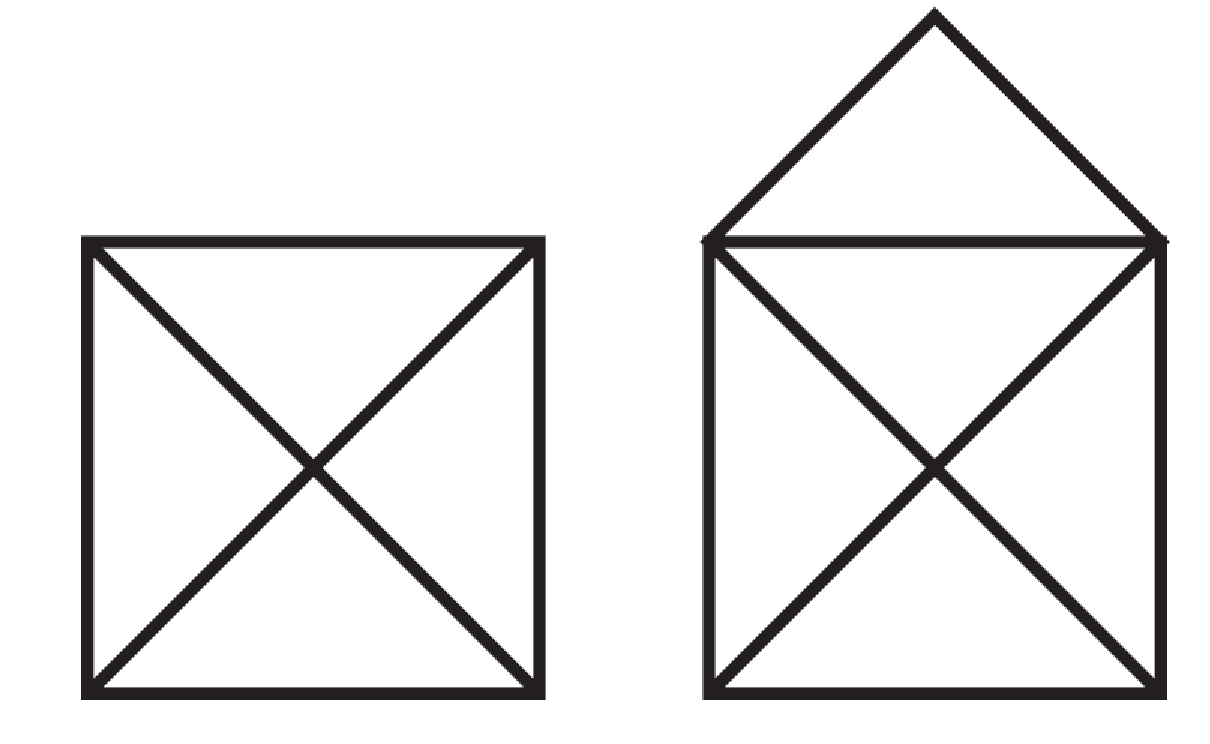
\includegraphics[scale=0.25]{LittleHouse.pdf}
\end{figure}
\column{0.5\textwidth}

Questions:
\itemb
\item Which graphs have Eulerian trails?
\item Which graphs have Eulerian tours?
\iteme
Now we give a complete answer.

\end{columns}
\end{frame}

\begin{frame}{Basic observations}

\bl[]{If $G$ has an Eulerian trail, then $G$ has at most one nontrivial component.}\vspace{0.3cm}

We call a component $\textit{trivial}$ if it contains only one vertex. If there are two or more components that are not trivial, then two edges in different components cannot be included in the same walk. Therefore we can restrict ourself to connected graphs WLOG.

\bl[]{If $G$ has an Eulerian trail, then it has at most two vertices of odd degree}

Let $v$ be neither the first or the last vertex on an Eulerian trail. Then the trail goes in and out $v$ the same number of times. As every edge is traversed exactly once, this implies that $d(v)$ must be even. Therefore only the first and the last vertices on the trail can have an odd degree.

\end{frame}

\begin{frame}{Basic observations}

\bl[]{If $G$ has an Eulerian trail that begins at a vertex $a$ and ends at a vertex $b$ with $a\neq b$, then vertices $a$ and $b$ have odd degree.}
The trail chooses an edge to leave $a$ as the first step of the walk. Then everytime the trail comes back to $a$ it must leave on an edge that it has not previously traversed.

\bl[]{If $G$ has an Eulerian tour, then all vertices have an even degree.}
In this case, every exit from a vertex $v$ we have an associated entrance. Since these all must happen on different edges, this implies $d(v)$ being even for every vertex of $G$.

\end{frame}

\begin{frame}{Basic observations}

\bl[]{If $G$ is a connected Eulerian graph, then $G$ has an Euler tour that begins/ends at any vertex.}
Let's assume that an Eulerian tour starts at $a\in V(G)$ and assume that the first visited vertex after $a$ is $b$:
\[
W=a\sim b\sim\dots\sim a.
\]
Then we can start the tour at $b$:
\[
W'=b\sim\dots\sim a\sim b.
\]
This way we can shift the tour to start at any vertex.

\end{frame}

\begin{frame}
\bl[Theorem]{Let $G$ be a connected graph. Then $G$ is Eulerian if and only if all vertices have even degree}
We prove this by induction on $|G|$.
We have seen ($\Rightarrow$) already. To prove ($\Leftarrow$), we will use strong induction on $|G|$.

~~~~\textbf{Basis case}: When $|G|=1$, let $v$ be the only point of $G$. Then it has no edges and therefore $(v)$ is trivially an Eulerian tour.

~~~~\textbf{Induction hypothesis}: Assume that the result is true for all $|G|=k$ with $k\leq n$. 

~~~~Let $G$ be a graph with $|G|=n+1$. Pick an arbitrary vertex $v$ and start forming a walk that does not traverse the same edge twice. If we reach a vertex where there are no more free edges to leave on, it must be the initial point because the degree of all vertices is even. Let $H$ be the longest such walk. FTSC assume it is not an Eulerian tour.

[...]
\end{frame}

\begin{frame}
\bl[Theorem]{Let $G$ be a connected graph. Then $G$ is Eulerian if and only if all vertices have even degree}
[...]

~~~~Consider the graph $G-E(P)$:
\begin{itemize}
\item  It does not contain any edges incident on $v$. 
\item All components have less vertices than $n$ and thus by the induction hypothesis, they containan Eulerian tours. 
\end{itemize}
Since $G$ is connected, there must be a component that contains a point $w$ that is on the walk $P$. Let us call the Eulerian tour of this component $Q$.

[...]
\end{frame}

\begin{frame}
\bl[Theorem]{Let $G$ be a connected graph. Then $G$ is Eulerian if and only if all vertices have even degree}
[...]

~~~~Consider the following walk. Follow $P$ from $v$ to $w$, then traverse $Q$ from $w$ to $w$, then traverse the rest of $P$ from $w$ to $v$. This walk is longer than $P$ and no edges are repeated along it which contradicts the maximality of $P$. $\Rightarrow\Leftarrow$.\qed
\end{frame}

\begin{frame}
\bl[Theorem]{Let $G$ be a connected graph. Then $G$ has an Eulerian trail if and only if the number of vertices with an odd degree is $0$ or $2$.}
~~~~Once again, we have already seen $(\Rightarrow)$. We use the previous theorem to prove $(\Leftarrow)$.
\begin{itemize}
\item If there are no odd vertices then there is an Eulerian tour which serves as an Eulerian trail too. 
\item If there are two odd vertices then 
\begin{itemize}
\item Add an extra edge connecting them (temporarily allow for parallel edges and note that it does not ruin the proof of the previous theorem). 
\item In the resulting graph every vertex has even degree and therefore there is an Eulerian tour. 
\item Now remove the extra edge and the tour breaks up to a trail.
\end{itemize}
\end{itemize}\qed
\end{frame}

\section{Coloring}

\begin{frame}{Statement of the problem}
\begin{columns}
\column{0.5\textwidth}
\includegraphics[scale=0.23]{MapColors.jpg}
\column{0.5\textwidth}
\bl[Statement of the problem]{Let $G$ be a graph. To each vertex of $G$, we wish to assign a color such that adjacent vertices receive different colors. We want to achieve this using as few colors as possible.}
\end{columns}\vspace{0.5cm}
We have seen applications:
\begin{columns}
\column{0.5\textwidth}
\itemb
\item Map coloring
\itemb
\item Vertices: Countries
\item Colors: Colors
\iteme
\iteme
\column{0.5\textwidth}
\itemb
\item Exam scheduling
\itemb
\item Vertices: Courses
\item Colors: Exams
\iteme
\iteme
\end{columns}
\end{frame}

\begin{frame}
\bl[Definition]{Let $G$ be a graph and let $k$ be a positive integer. A \textbf{$k$-coloring} of $G$ is a function
\[
f:V(G)\to\{1,2,\dots,k\}
\]
We call this coloring \textbf{proper} provided
\[
\forall xy\in E(G),\qquad f(x)\neq f(y).
\]
If a graph has a proper $k$-coloring, we call it $k$-colorable.}
\itemb
\item For a vertex $v$, the value $f(v)$ is its color.
\item $\{1,\dots, k\}$ is our palette.
\item The proper coloring means that for any edge, the two endpoints are colored differently.
\item The definition does not require that we use all colors (or in other words that $f$ is onto).
\iteme
\end{frame}

\begin{frame}
\bl[Definition]{Let $G$ be a graph. The smallest positive integer $k$ for which $G$ is $k$-colorable is called the \textbf{chromatic number} of $G$. The chromatic number of $G$ is denoted $\chi(G)$.}
For example, consider $K_n$.
\itemb
\item We can properly color $K_n$ using $n$ colors.
\item We cannot do better than that because every vertex is adjacent to every other!
\iteme
Therefore $\chi(K_n)=n$.
\bl[Proposition]{If $G$ is a subgraph of a graph $H$, then $\chi(G)\leq\chi(H)$.}
Given a proper coloring of $H$, let every vertex $v\in V(G)$ have the same color as it does in $H$. This results in a proper coloring of $G$.\qed
\end{frame}

\begin{frame}{Easy bounds}
\bl[Proposition]{Let $G$ be a graph with maximum degree $\Delta$. Then $\chi(G)\leq \Delta+1$.}
Note that one can color naively one vertex after another. Since every point has at most $\Delta$ neighbors, there is always a color on the palette of size $\Delta+1$ that is different from all the neighbor's colors.\qed
\bl[Proposition]{Let $G$ be a graph with at least one edge. Then $\chi(G)\geq 2$.}
Let $xy\in E(G)$ be an edge. Then $x$ and $y$ have to have different colors.\qed
\end{frame}

\begin{frame}{Chromatic number of cycles}
\begin{columns}
\column{0.4\textwidth}
\includegraphics[scale=0.23]{CycleChrom.jpg}
\column{0.6\textwidth}
\itemb
\item If $n$ is even, then the black-white-black pattern works.
\item If $n$ is odd, then this does not work and we need one more color.
\iteme
\end{columns}\vspace{0.5cm}
\[
\chi(C_n)=\left\{\begin{array}{ll}
2&\textrm{if $n$ is even},\\
3&\textrm{if $n$ is odd}
\end{array}\right.
\]
Note that when $n$ is odd, $\chi(C_n)=3$, even though $d(v)=2$ for every $v\in V(G)$.
\end{frame}

\begin{frame}{One and two colorable graphs}
\bl[Proposition]{A graph $G$ is one colorable if and only if it is edgeless}
Follows from our easy lower bound.\qed
\bl[Definition]{A graph $G$ is called \textbf{bipartite} provided it is $2$-colorable}
Let $G$ be a bipartite graph and select a proper two coloring $f$. Let
\itemb
\item Let $X=\{v\in V(G): f(v)=1\}$
\item Let $Y=\{v\in V(G): f(v)=2\}$
\iteme
Then $\{X,Y\}$ is a partition of $V(G)$. If $e\in E(G)$, then one of its endpoints is in $X$, and the other one is in $Y$.
\bl[]{ $\{X,Y\}$ is called a bipartition of $G$.
}
\end{frame}

\begin{frame}{Examples of bipartite graphs}
\itemb
\item $C_n$ is bipartite for every even $n$.
\item Trees
\iteme
\bl[Proposition]{Trees are bipartite}
~~~~We prove this by induction on the number of vertices.

~~~~\textbf{Basis case:} Clearly a tree with one vertex is bipartite as $\chi(K_1)=1\leq 2$.

~~~~\textbf{Induction hypothesis:} Every tree with $n$ vertices is bipartite.

~~~~Let $T$ be a tree with $n+1$ vertices and let $v$ be a leaf. Let $T'=T-v$. Since $T'$ is a tree with $n$ vertices, it is bipartite by the induction hypothesis. Let $f$ be a proper $2$-coloring of $T'$. 

~~~~Now consider $v$-s only neighbor $w$. Whatever $f(w)$ is, assign $v$ the other color. This gives a proper two coloring of $T$. \qed
\end{frame}

\begin{frame}{Complete bipartite graphs}
\begin{columns}
\column{0.3\textwidth}
\begin{figure}
\centering
\includegraphics[scale=0.25]{ComplBipart.jpg}
\caption{This is $K_{4,3}$.}
\end{figure}
\column{0.7\textwidth}
\bl[Definition]{Let $n,m$ be positive integers. The \textbf{complete bipartite graph} $K_{n,m}$ is a graph whose vertices can be partitioned $V=X\cup Y$ such that
\itemb
\item $|X|=n$,
\item $|Y|=m$,
\item $xy\in E(K_{n,m})$ for all $x\in X$ and $y\in Y$.
\item No edge has both its endpoints in either $X$ or $Y$.
\iteme}
\end{columns}

\end{frame}

\begin{frame}{Criterion for bipartite-ness}
How can one check whether a graph is bipartite?
\itemb
\item Showing that a graph is bipartite is easy. Just start coloring points alternating the colors and if it works the graph is bipartite.
\item If it is not bipartite than choosing two adjecent points, assinging them different colors and then coloring with alternating colors will break down.
\iteme
Alternatively, this can be seen to be captured by the following theorem.
\bl[Theorem]{A graph is bipartite if and only if it does not contain an odd cycle.}\vspace{-0.3cm}
\center\textcolor{red}{However no such criterion is known for more than two colors.}
\end{frame}

\section{Planar graphs}

\begin{frame}{Planar graphs}
\bl[Theorem]{A \textbf{planar graph} is a graph that can be drawn in the plane without any two edges crossing each other.}
Examples of non-planar graphs:\vspace{-0.2cm}
\begin{columns}
\column{0.65\textwidth}
\begin{figure}
\centering
\includegraphics[scale=0.5]{kuratowski2.jpg}
\end{figure}
\column{0.35\textwidth}
\bl[Theorem (Kuratowski)]{A graph $G$ is planar if and only if it does not contain a subdivision of $K_5$ or $K_{3,3}$ as a subgraph.}

\end{columns}\vspace{0.2cm}
(A subdivision of a graph $G$ is formed from $G$ by replacing edges with paths.)\end{frame}

\begin{frame}{Coloring of planar graphs}
To prove that for any planar graphs $G$, $\chi(G)\leq 6$ is not hard. Neither is to show that $\chi(G)\leq 5$ just a little lengthier. However the proof of the following theorem is hundreds of pages long.\vspace{0.5cm}

\bl[The $4$ coloring theorem]{If $G$ is a planar graph, then $\chi(G)\leq 4$.}\vspace{0.5cm}

For example, graphs coming from maps are planar and therefore $4$-colorable.
\end{frame}


\end{document}